\newpage
\section[Differentiation]{\hyperlink{toc}{Differentiation}}

\subsection{Derivatives}
\begin{definition}{Derivatives}{5.1}
    Let $f: [a, b] \mapsto \RR$, and $x \in [a, b]$. We then define the \textbf{derivative} of $f$ at $x$ as:
    \begin{align*}
        f'(x) = \lim_{t\rightarrow x} \frac{f(t) - f(x)}{t - x}
    \end{align*}
    If the limit exists. Alternative notations for the derivative are given by:
    \begin{align*}
        \dpd{f}{x}(x) \text{ or } \dod{}{x}f(x) \text { or } \left.\dod{}{y}f(x)\right|_{y = x}
    \end{align*}
\end{definition}
As an interpretation of the derivative, take $[a, b]$ to be a metric space, with $x$ a limit point of $[a, b] \setminus \set{x}$. Then, $g(t) = \frac{f(t) - f(x)}{t - x}$ is a function from $[a, b] \setminus \set{x} \mapsto \RR$. If $x \in (a, b)$, then the above definition of the derivative agrees with the definition of $f'(x)$ from first year calculus. If $x = a$ or $x = b$, then the above definition agrees with the definition of the one-sided derivative from first year calculus. Note that we will not discuss in this class cases where the domain gets more complicated (i.e. not just closed intervals of $\RR$).

\begin{theorem}{}{5.2}
    Let $f:[a,b] \mapsto \RR$, let $x \in [a, b]$, and suppose $f'(x)$ exists. Then, $f$ is continuous at $x$.
\end{theorem}
\begin{nproof}
    For $t \neq x$, we can write:
    \begin{align*}
        f(t) = f(x) + (f(t) - f(x)) = f(x) + \frac{f(t) - f(x)}{t - x}(t - x)
    \end{align*}
    Taking the limit of $t \rightarrow x$, we then have that:
    \begin{align*}
        \lim_{t \rightarrow x} f(t) = \lim_{t \rightarrow x} \left(f(x) + \frac{f(t) - f(x)}{t - x}(t - x) \right) = \lim_{t \rightarrow x} f(x) + \lim_{t \rightarrow x} \frac{f(t) - f(x)}{t - x} \lim_{t \rightarrow x} (t - x)
    \end{align*}
    Where in the last line we invoke Theorem \ref{thm:4.4}. Evaluating the limits on the RHS by using the existence of the derivative of $f$ at $x$, we have
    \begin{align*}
        \lim_{t \rightarrow x} f(t) = f(x) + f'(x)\cdot (0) = f(x)
    \end{align*}
    So we conclude that $f$ is continuous at $x$ by Theorem \ref{thm:4.6}. \qed
\end{nproof}
The interpretation is that differentiability at $x \in (a, b)$ implies continuity of $f$ at $x$, and the left/right differentiability of $f$ at $a/b$ implies the left/right continuity of $f$ at $a/b$. We have wrapped the proof of all these cases into one!

Note that the converse of the above theorem is not true. As a simple example, take $f(x) = \abs{x}$ on $[-1, 1]$, which is continuous at $x = 0$ (it can be verified that $\lim_{x \rightarrow 0}f(x) = f(0) = 0$) but is not differentiable there (the left/right handed limits of the difference quotient do not agree and hence the derivative does not exist). In Chapter 7, we will construct a function that is continuous everywhere and differentiable nowhere!

NWe will now proceed to prove a series of theorems that have been seen in first year, but using our new/rigorous definitions.

\begin{theorem}{Sum, Product, and Quotient Rules}{5.3}
    Let $f, g: [a, b] \mapsto \RR$. Let $x \in [a, b]$ and suppose $f$ and $g$ are differentiable at $x$. Then, $f + g$, $f - g$, $f\cdot g$ are differentiable at $x$, and so is $\frac{f}{g}$ provided $g(x) \neq 0$. Furthermore:
    \begin{enumerate}
        \item $(f+g)'(x) = f'(x) + g'(x)$
        \item $(fg)'(x) = f'(x)g(x) + f(x)g'(x)$
        \item $\left(\frac{f}{g}\right)'(x) = \frac{f'(x)g(x) - f(x)g'(x)}{(g(x))^2}$
    \end{enumerate}
\end{theorem}
\begin{nproof}
    \begin{enumerate}
        \item Follows immediately from the additive property of limits (Theorem \ref{thm:4.4}).
        \item Let $h = fg$. We then have that:
        \begin{align*}
            h(t) - h(x) = f(t)\left[g(t) - g(x)\right] + g(x)\left[f(t) - f(x)\right]
        \end{align*}
        For $t \neq x$, we can divide both sides by $t-x$ to obtain:
        \begin{align*}
            \frac{h(t) - h(x)}{t - x} = f(t)\frac{g(t) - g(x)}{t-x} + g(x)\frac{f(t) - f(x)}{t - x}
        \end{align*}
        Taking the limit of $t \rightarrow x$ on both sides, we obtain:
        \begin{align*}
            h'(x) = f(x)g'(x) + f'(x)g(x)
        \end{align*}
        as desired.
        \item Let $h(t) = \frac{f(t)}{g(t)}$. Then:
        \begin{align*}
            h(t) - h(x) &= \frac{f(t)}{g(t)} - \frac{f(x)}{g(x)}
            \\ &= \frac{1}{g(t)g(x)}\left(f(t)g(x) - g(t)f(x)\right)
            \\ &= \frac{1}{g(t)g(x)}\left[g(x)\left(f(t) - f(x)\right) - f(x)\left(g(t) - g(x)\right)\right]
        \end{align*}
        For $t \neq x$, we can divide both sides by $t - x$ to get:
        \begin{align*}
            \frac{h(t) - h(x)}{t - x} = \frac{1}{g(t)g(x)}\left[g(t)\frac{f(t) - f(x)}{t - x} - f(x)\frac{g(t) - g(x)}{t - x}\right]
        \end{align*}
        Taking the limit as $t \rightarrow x$ on both sides, we obtain the desired expression. \qed
    \end{enumerate}
\end{nproof}

\newpage 
\noindent As an exercise, one can prove by induction (applying 5.3(b)) that $(f_1f_2f_3\ldots f_n)'(x)$ (where $f_i: [a, b] \mapsto \RR$ and each $f_i'(x)$ exists) is given by:
\begin{align*}
    f_1'(x)f_2(x)\ldots f_n(x) + \cdots + f_1(x)f_2(x)\ldots f'_n(x).
\end{align*}
Note that as a corollary of this, we get that if $f(x) = x^n$, then $f'(x) = nx^{n-1}$ and we hence recover the familiar power rule from first year calculus!

\setcounter{rudin}{4}
\begin{theorem}{Chain Rule}{5.5}
    Let $f: [a, b] \mapsto \RR$, $x \in [a, b]$, and suppose $f$ is differentiable at $x$. Suppose furthermore that $f([a, b])$ is contained in some interval $I$. Let $g: I \mapsto \RR$ and suppose $g$ is differentiable at $f(x)$. Then, $g \circ f: [a, b] \mapsto \RR$ is differentiable at $x$, and furthermore:
    \begin{align*}
        (g \circ f)'(x) = g'(f(x))f'(x)
    \end{align*}
\end{theorem}
\begin{nproof}
    Define $h(t) = g \circ f(t)$ for $a \leq t \leq b$, $t \neq x$. We cna then write:
    \begin{align*}
        f(t) - f(x) = (t-x)\left[f'(x) + u(t)\right]
    \end{align*}
    For a function $u(t)$ with $\lim_{t \rightarrow x} u(t) = 0$. Now defining $y = f(x)$, we write:
    \begin{align*}
        g(s) - g(y) = (s-y)\left[g'(y) + r(s)\right]
    \end{align*}
    For a function $r(s)$ with $\lim_{s \rightarrow y}r(s) = 0$. Hence, we have that:
    \begin{align*}
        h(t) - h(x) &= g(f(t)) - g(f(x))
        \\ &= \left(f(t) - f(x)\right)\left(g'(y) + r(s)\right)
        \\ &= (t- x)\left[f'(x) + u(t)\right]\left(g'(y) + r(s)\right)
    \end{align*}
    Dividing both sides by $t - x$, we obtain:
    \begin{align*}
        \frac{h(t) - h(x)}{t - x} = \left[f'(x) + u(t)\right]\left(g'(y) + r(s)\right)
    \end{align*}
    We now take the limit of $t \rightarrow x$ on both sides. $\lim_{t \rightarrow x} u(t) = 0$, and $f$ is differentiable and hence continuous at $x$, so $s = f(t) \rightarrow y$ as $t \rightarrow x$. Thus, $r(s) \rightarrow 0$ as $t \rightarrow x$, and in conclusion:
    \begin{align*}
        h'(x) = (g \circ f)'(x) =  f'(x)g'(y) = g'(f(x))f'(x)
    \end{align*}
    as desired. \qed
\end{nproof}


\subsection{MVT}

\setcounter{rudin}{6}
\begin{definition}{Local Maxima/Minima}{5.7}
    Let $X$ be a metric space. Let $f: X \mapsto \RR$, and let $x \in X$. We say that $x$ is a \textbf{local maximum} of $f$ if there exists $\delta > 0$ such that $f(y) \leq f(x)$ for all $y \in N_{\delta}(x)$. A \textbf{local minimum} is defined similarly, with $f(y) \geq f(x)$ instead.
\end{definition}
\noindent For a metric space $X$ equipped with the discrete metric, all points $x \in X$ are simultaneously local maxima and minima. To see this, take any $0 < \delta \leq 1$. 

\begin{theorem}{}{5.8}
    Let $f: [a, b] \mapsto \RR$. Let $x \in [a, b]$ and suppose that $f'(x)$ exists, and $f$ is either a local maximum or local minimum of $f$. Then, $f'(x) = 0$. 
\end{theorem}
\begin{nproof}
    Suppose $x$ is a local minimum. Then, there exists $\delta > 0$ such that $N_{\delta}(x) \subset [a, b]$, and $f(y) \geq f(x)$ for all $y \in N_{\delta}(x)$. Thus, if $x < y < x + \delta$, then:
    \begin{align*}
        \frac{f(y) - f(x)}{y - x} \geq 0 \implies f'(x) \geq 0
    \end{align*}
    Conversely, if $x - \delta < y < x$, then:
    \begin{align*}
        \frac{f(y) - f(x)}{y - x} \leq 0 \implies f'(x) \leq 0
    \end{align*}
    So taken together we obtain that $f'(x) = 0$. An identical argument is used for the case of a local maximum. \qed
\end{nproof}

\begin{ntheorem}{: Rolle's Theorem}{}
    Let $f: [a, b] \mapsto \RR$ be continuous, and suppose $f$ is differentiable on $(a, b)$. If $f(a) = f(b)$, then there exists $x \in (a, b)$ such that $f'(x) = 0$.
\end{ntheorem}
\begin{nproof}
    Since $[a, b]$ is compact and $f$ is continuous, by the EVT (Theorem \ref{thm:4.16}) $f$ attains its maximum on $[a, b]$, that is, there exists $c \in [a, b]$ such that $f(y) \leq f(x)$ for all $y \in [a, b]$. If $c \in (a, b)$, then by Theorem \ref{thm:5.8}, $f'(c) = 0$ and we are done. Next, suppose $c = a$ or $c = b$. Again by the EVT, $f$ attains its minumum on $[a, b]$, that is, there exists $d \in [a, b]$ such that $f(y) \geq f(d)$ for all $y \in [a, b]$. If $d \in (a, b)$, then by Theorem \ref{thm:5.8}, $f'(d) = 0$ and we are done. Suppose then that $d = a$ or $d = b$. Since $f(a) = f(b)$, we therefore obtain that $f(a) = f(b) = f(c) = f(d)$ and the maximum/minimum values agree. Hence, $f(y) = f(a)$ for all $y \in [a, b]$, so $f'(y) = 0$ for all $y \in [a, b]$. So, the desired $x$ may be any point in $[a, b]$. \qed
\end{nproof}

\begin{figure}[htbp]
    \centering
    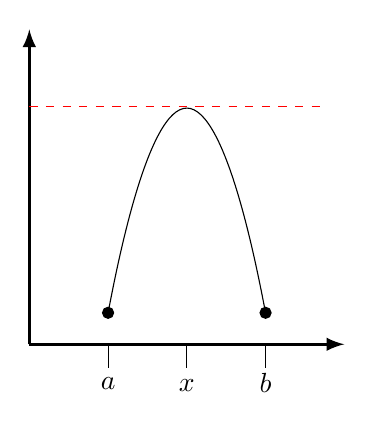
\begin{tikzpicture}[scale = 2]
        \draw[-latex, very thick] (0, 0) -- (0, 2);
        \draw[-latex, very thick] (0, 0) -- (2, 0);
        \draw[] (1, 1.5) parabola (0.5, 0.2);
        \draw[] (1, 1.5) parabola (1.5, 0.2);
        \filldraw[] (0.5, 0.2) circle (1pt);
        \filldraw[] (1.5, 0.2) circle (1pt);
        \draw[dashed, red] (0, 1.51) -- (1.85, 1.51);
        \draw[] (0.5, 0) -- (0.5, -0.15);
        \node[below] at (0.5, -0.15) {$a$};
        \draw[] (1.5, 0) -- (1.5, -0.15);
        \node[below] at (1.5, -0.12) {$b$};
        \draw[] (1, 0) -- (1, -0.15);
        \node[below] at (1, -0.16) {$x$};
    \end{tikzpicture}
    
    \caption{A simple parabolic function that demonstrates Rolle's Theorem.}
    \label{fig21}
\end{figure}

\newpage 
\setcounter{rudin}{9}
\begin{theorem}{Mean Value Theorem}{5.10}
    Let $f: [a, b] \mapsto \RR$ be continuosu and differentiable on $(a, b)$. Then, there exists $x \in (a, b)$ such that $f(b) - f(a) = f'(x)(b - a)$.
\end{theorem}
\noindent The visual interpretation of this theorem is that there exists $x \in (a, b)$ such that the slope of the tangent line to $f$ at $x$ is equal to the secant line slope between $(a, f(a))$ and $(b, f(b))$. The idea of the proof is to rotate one's head such that the sectant line is horizontal; one is then able to apply Rolle's Theorem!

\begin{nproof}
    Define $h(y) = f(y) = \frac{f(b) - f(a)}{b - a}(y - a)$. $h$ is continuous on $[a, b]$ and differentiable on $(a, b)$ (being a sum of continuous/differentiable functions). We have that $h(a) = f(a) - 0 = f(a)$, and $h(b) = f(b) - \frac{f(b) - f(a)}{b - a}(b - a) = f(a)$. Applying Rolle's Theorem to $h$, there exists $x \in (a, b)$ such that $h'(x) = 0$. Therefore, $h'(x) = 0 = f'(x) - \frac{f(a) - f(b)}{b - a} = 0$, and we conclude that $f(b) - f(a) = f'(x)(b - a)$ for some $x \in (a, b)$. \qed
\end{nproof}

\begin{figure}[htbp]
    \centering
    \begin{tikzpicture}[scale=2]
    \draw[-latex, very thick] (0, 0) -- (0, 2);
    \draw[-latex, very thick] (0, 0) -- (2, 0);
    \draw [] (0.5 , 0.25) to [ curve through ={(1, 1.25)}] (1.5,1.5);
    \filldraw[] (0.5, 0.25) circle (1pt);
    \filldraw[] (1.5, 1.5) circle (1pt);
    \draw[dashed] (0.5, 0.25) -- (1.5, 1.5);
    \draw[dashed, red] (0, 0.075) -- (1, 1.325) -- (1.42,1.85);
    \draw[] (0.5, 0) -- (0.5, -0.15);
    \node[below] at (0.5, -0.15) {$a$};
    \draw[] (1.5, 0) -- (1.5, -0.15);
    \node[below] at (1.5, -0.12) {$b$};
    \draw[] (0.775, 0) -- (0.775, -0.15);
    \node[below] at (0.775, -0.16) {$x$};
    \end{tikzpicture}
    \caption{A simple continuous function that demonstrates the MVT.}
    \label{fig22}
\end{figure}


\begin{theorem}{}{5.11}
    Let $f: [a, b] \mapsto \RR$ be differentiable on $(a, b)$. Then:
    \begin{enumerate}
        \item If $f'(x) \geq 0$ for all $x \in (a, b)$, then $f$ is monotonically increasing.
        \item If $f'(x) = 0$ for all $x \in (a, b)$, then $f$ is constant. 
        \item If $f'(x) \leq 0$ for all $x \in (a, b)$, then $f$ is monotonically decreasing.
    \end{enumerate} 
\end{theorem}
\begin{nproof}
    If $a < x < y < b$, by the mean value theorem, there exists $z \in (x, y)$ such that:
    \begin{align*}
        f(y) - f(x) = f'(z)(y - x)
    \end{align*}
    Note that $y - x > 0$ by construction. 
    \begin{enumerate}
        \item If $f'(x) \geq 0$ for all $x \in (a, b)$, then $f'(z) \geq 0$, showing that $f(y) - f(x) \geq 0$ and hence that $f$ is monotonically increasing. 
        \item If $f'(x) = 0$ for all $x \in (a, b)$, then $f'(z) = 0$, showing that $f(y) - f(x) = 0$ and hence that $f$ is constant on $(a, b)$.
        \item If $f'(x) \leq 0$ for all $x \in (a, b)$, then $f'(z) \leq 0$, showing that $f(y) - f(x) \leq 0$ and hence that $f$ is monotonically decreasing. \qed
    \end{enumerate}
\end{nproof}

\subsection{Taylor's Theorem}
\setcounter{rudin}{13}
\begin{definition}{Higher Order Derivatives}{5.14}
If $f$ is differentiable in a neighbourhood of $x$, then we may compute a second order derivative:
\begin{align*}
    \lim_{t \rightarrow x} \frac{f'(t) - f'(x)}{t - x} = (f')'(x) = f''(x)
\end{align*}
We can then continue this process to obtain $f^{(3)}(x), f^{(4)}(x), \ldots, f^{(n)}(x)$. 
\end{definition}
\begin{ndef}{: \texorpdfstring{$C^n(I, \RR)$}{Cn(I, R)}}{}
    If $f$ is continuous in $I$, we can write $f \in C^{0}(I, \RR)$. If $f$ is differentiable in a neighbourhood $I$ and the derivative $f'$ is continuous in $I$, then we write $f \in C^{1}(I, \RR)$. In general, $f \in C^{n}(I, \RR)$ denotes the $n$th derivative of $f$ is continuous in $I$. Note that where it is clear from context, we may drop the $\RR$ and just write $C^n(I)$. 
\end{ndef}
\noindent Recall that for a function $f$ continuous and differentiable on $(x_0, x)$, the Mean Value Theorem proved the existence of some $\tilde{x}$ such that:
\begin{align*}
    f(x) = f(x_0) + f'(\tilde{x})(x - x_0)
\end{align*}
This gives us a natural method to build up approximations for functions; we can start with a constant approximation $f(x_0)$, then add a linear term $f'(\tilde{x})(x - x_0)$, then add on a quadratic term $(x - x_0)^2$ and so on. The following theorem gives us a way to construct these approximations and bound their error.

\begin{theorem}{Taylor's Theorem}{5.15}
    Let $I$ be a neighbourhood of $x_0$, and $f \in C^p(I)$. Then, for any $n < p$, we have that:
    \begin{align*}
        f(x) = \sum_{j=0}^n \frac{f^{(j)}(x_0)}{j!}(x- x_0)^j + \frac{f^{(n+1)}(\tilde{x})}{(n+1)!}(x - x_0)^{n+1}
    \end{align*}
    Where $\tilde{x} = x_0 + \lambda(x - x_0)$ for some $\lambda \in (0, 1)$ (i.e. $\tilde{x} \in (x_0, x)$). Note that $\tilde{x}$ depends on $x, x_0$, and $n$. 
\end{theorem}
\begin{nproof}
    For $n = 0$, the claim reduces to the Mean Value Theorem. Then, let $n \geq 1$. Let $A$ be a constant that depends on $x, x_0$, and $n$, and let $P_n(x) = \sum_{j=0}^n \frac{f^{(j)}(x_0)}{j!}(x-x_0)^j$. Then, we can write:
    \begin{align*}
        f(x) = P_n(x) + A(x-x_0)^{n+1}
    \end{align*}
    We need to show that we can express $A$ as relating to the derivative, namely, that there exists $\tilde{x}$ such that $A = \frac{f^{(n+1)}(\tilde{x})}{(n+1)!}$. Let $g(t) = f(t) - P_n(t) - A(t - x_0)^{n+1}$ with $t \in I$. Then, $g \in C^{p}(I)$. For $n < p$, we then have that:
    \begin{align*}
        g^{(n+1)}(t) = f^{(n+1)}(t) - 0 - A(n+1)!(t - x_0)
    \end{align*}
    We claim that there exists $\tilde{x} \in (x_0, x)$ such that $g^{(n+1)}(\tilde{x}) = 0$. To see this, consider that $P^{(j)}(x_0) = f^{(j)}(x_0)$ for $j = 0, 1, \ldots, n$, so $g(x_0) = 0$, and furthermore:
    \begin{align*}
        g'(x_0) = g''(x_0) = g^{(3)}(x_0) = \ldots = g^{(n)}(x_0) = 0
    \end{align*}
    Moreover y the choice of $n$, we have that $g(x) = 0$. Hence, by Rolle's Theorem, there exists a point $x_1$ between $x_0$ and $x$ such that $g'(x_1) = 0$. Similarly, repeating the argument above, there exists an $x_2$ between $x_0$ and $x_1$ such that $g''(x_2) = 0$. Repeating this process up to $g^{(n)}$, we have that $g^{(n)}(x_n) = 0$, for some $x_0 < x_{n} < x_{n-1} < \cdots < x$ and in turn, there exists $x_{n+1} \in (x_0, x_n)$ such that $g^{(n+1)}(x_{n+1}) = 0$. Setting $\tilde{x} = x_{n+1}$, the claim is shown. \qed
\end{nproof}

\noindent As an example, we consider the Taylor series of the function $f(x) = \cos(x)$ (We will formally define this function later on, but for now, let us assume its familar properties and derivatives). We then have that:
\begin{align*}
    f^{(j)}(0) = \begin{cases}
        (-1)^m & \text{if $j = 2m$}
        \\ 0 & \text{if $j = 2m + 1$}
    \end{cases}
\end{align*}
If we have the sum run from $j = 0$ to some $j = n$, let us then try to estimate the rest. Let $\tilde{x} \in (0, x)$. Then, letting the error term be represented by $\e$, we have that:
\begin{align*}
    \e = \abs{\frac{f^{(n+1)}(\tilde{x})}{(n+1)!}(x-x_0)^{n+1}} \leq \frac{\abs{x}^{n+1}}{(n+1)!} 
\end{align*}
And we observe that $\linf \frac{\abs{x}^{n+1}}{(n+1)!} = 0$ and hence the error $\e$ goes to zero in the $n \rightarrow \infty$ limit. Therefore, the difference between $\cos(x)$ and its Taylor polynomial vanishes quickly for any $x$, and the Taylor series converges for all $x$. Taking the limit of the sum, we have that:
\begin{align*}
    f(x) = \cos(x) = \linf \left(P_{n}(x) + \frac{f^{(n+1)}(x_0)}{(n+1)!}(x - x_0)^{n+1}\right) = \sum_{j=0}^\infty \frac{(-1)^{2m}}{m!}x^{2m} = 1 - \frac{x^2}{2} + \frac{x^4}{4} - \frac{x^6}{6} + \ldots
\end{align*}
A question of interest might be how many terms do we need in the Polynomial such that our error is less than $10^{-6}$, say, for estimating the value of $\cos(\frac{\pi}{12})$. In other words, we want to find the $m$ such that:
\begin{align*}
    \frac{1}{2m!}\left(\frac{\pi}{12}\right)^{2m} \leq 10^{-6}
\end{align*}
Rearranging, we require:
\begin{align*}
    (2m)!\left(\frac{12}{\pi}\right)^{2m} > 10^6
\end{align*}
Making a table of the value of the LHS as a function of $m$, we have:
\begin{table}[htbp]
    \centering\begin{tabular}{c|c}
    $m$ & $(2m)!\left(\frac{12}{\pi}\right)^{2m}$
    \\ \hline
    1 & $\approx 29$
    \\ 2 & $\approx 5110$
    \\ 3 & $\approx 2.23 \times 10^{6}$
    \end{tabular}
\end{table}
So we see that three terms are sufficient for a good approximation in this case (and as stated before, the series converges very quickly)!

A natural question of interest is the convergence of the sum in the $N \rightarrow \infty$ limit, that is, the convergence of the power series $\sum_{n = 0}^\infty \frac{f^{(n)}(x_0)}{n!}(x - x_0)^n$. We are also interested are interested for when $f(x) = \sum_{n = 0}^\infty \frac{f^{(n)}(x_0)}{n!}(x - x_0)^n$ holds (that is, when is a function equal to its Taylor series)? These turn out to be distinct questions; in particular, there are functions whose power series converge for all $x$ but are equal to their power series nowhere (except at $x_0$ where equality must hold). This motivates the following definition:
\begin{ndef}{: Analyticity}{}
    A function $f$ is \textbf{analytic} if $f(x) = \sum_{n=0}^\infty \frac{f^{(n)}(x_0)}{n!}(x - x_0)^n$ in a neighbourhood of $x_0$.
\end{ndef}
\noindent To motivate this definition, it will help to study a function which is \textit{not} analytic. Consider the function:
\begin{align*}
    f(x) = \begin{cases}
        \exp(-\frac{1}{x}) & x > 0
        \\ 0 & x \leq 0
    \end{cases}
\end{align*}
\begin{figure}[htbp]
    \centering
    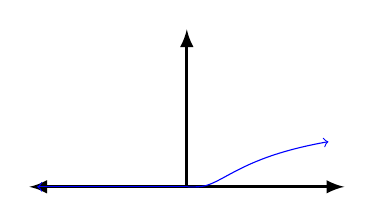
\begin{tikzpicture}
        \draw[latex-latex, very thick] (-2, 0) -- (2, 0);
        \draw[-latex, very thick] (0, 0) -- (0, 2);
        \draw[<-, blue] (-1.9, 0) -- (0.02, 0);
        \draw[->, blue, smooth, samples = 100, domain=0.01:1.8, variable = \x] plot(\x, {exp(-1/\x)});
    \end{tikzpicture}
    \caption{Plot of $f$.}
    \label{fig23}
\end{figure}

\noindent $f$ is continuous everywhere by construction. It is infinitely differentiable at $x = 0$, but it is only equal to its Taylor series around $x_0 =0$ for $x \leq 0$. To see this, we observe that:

\begin{align*}
    f'(x) = \frac{1}{x^2}\exp(-\frac{1}{x})
\end{align*}
\begin{align*}
    f^{(n)}(x) = \frac{P_n(x)}{x^{2n}}\exp(-\frac{1}{x})
\end{align*}
We have that $f^{(n)}(x) \rightarrow 0$ as $x \rightarrow 0$ for all $n$ as the exponential dominates the polynomial singularity. We hence have that $f \in C^\infty$. The taylor polynomial at $x_0 = 0$ however, as we have that $f(0) = 0$ and $f^{(n)}(0) = 0$, leading to:
\begin{align*}
    \sum_{n=0}^N \frac{f^{(n)}(0)}{n!}x^n = 0
\end{align*}
for all $N$. We therefore have that the series converges for all $x$, but is only equal to $f$ for $x \leq 0$; hence it is not analytic (as there exists no neighbourhood around $x_0= 0$ for which $f$ is equal to its Taylor series). 

We now consider a function $\chi(x)$ defined as $\chi(x) = \frac{f(x)}{f(x) + f(1 - x)}$. This function is alsoz continuous, its denominator is never zero, and $\chi \in C^\infty$. We observe that $\chi(x) = 0$ for $x \leq 0$ and $\chi(x) = 1$ for $x \geq 1$, and overall the function looks much like a step function:

\begin{figure}[htbp]
    \centering
    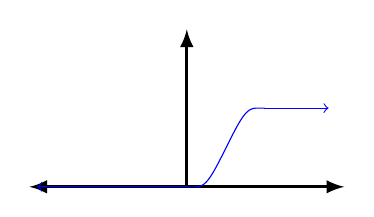
\begin{tikzpicture}
        \draw[latex-latex, very thick] (-2, 0) -- (2, 0);
        \draw[-latex, very thick] (0, 0) -- (0, 2);
        \draw[<-, blue] (-1.9, 0) -- (0.02, 0);
        \draw[blue, smooth, samples = 100, domain=0.01:0.99, variable = \x] plot(\x, {exp(-1/\x)/(exp(-1/\x) + exp(-1/(1-\x)))});
        \draw[blue, ->] (0.98, 1) -- (1.8, 1);
    \end{tikzpicture}
    \caption{Plot of $\chi$.}
    \label{fig24}
\end{figure}
Indeed, this function can be used as a ``cutoff''/``switch'' function that behaves much like a step function (except it is infinitely differentiable).

A question becomes whether such a function could be analytic. The answer turns out to be no, and the proof we leave as an exercise. As a sketch, consider an analytic function $g$ such that $g(x) = 0$ for $x \leq x_0$ and $g(x) \neq 0$ for $x > x_0$. One can derive a contradiction by considering the Taylor series expansion about $x_0$ and then using the assumed analyticity of $g$. 

Note that in a sense, Taylor's Theorem is the culmination of a sequence of theorems we have proven in the course. Roughly, the sequence was as follows:
\begin{enumerate}[1)]
    \item $f: X \mapsto Y$ and $K \subset X$, then $f(K)$ compact (Theorem \ref{thm:4.14})
    \item Extreme Value Theorem: If $f: X \mapsto \RR$ with $f$ continu$(X, \tau)$ and $(Y, \rho)$ ous and $K$ compact, then $f$ realizes its supremum and infimum on $K$. (Theorem \ref{thm:4.16})
        
    \item Rolle's Theorem
    \item Mean Value Theorem (Theorem \ref{thm:5.10})
    \item Taylor's Theorem (Theorem \ref{thm:5.15})
\end{enumerate}
A question that arises is could we have gone through this sequence of proofs with just the rational numbers ($\QQ$)? The intuitive answer is no, but it may be interesting to see where along this chain the logic breaks down.

The first step that looks immediately questionable is step 2; the supremum/infimum is not well-defined for all subsets of $\QQ$, so we might be able to find a breakdown there. To this end, we consider the set $A = \set{q \in \QQ: q > 0, q^2 < 2}$ that arises in Example \ref{exam:1.1a} and try to find a function $f: K \mapsto \QQ$ with $K \subset \QQ$ compact such that $f(K) = A$. An idea would be to try $f(x) = \sqrt{x}$, with $K = \set{q \in \QQ: \exists r: r^2 = q} \cap [0, 2]$ but this doesn't work as $K$ is not compact. Trying another attempt, $K = [1, 2] \cap \QQ$ with $f(x) = \sin(x)$ does not work either as $\sin(x)$ is not necessarily rational, and moreover, $[1, 3] \cap \QQ$ is not a compact set as not all Cauchy sequences in $S$ converge! Another attempt would be $K = [1, 2] \cap \QQ = X$ with $f(q) = \abs{q^2 - 2}$ where it would seem as though $f(K) = \set{r \in \QQ: 0 < r \leq 2}$ provides a good counterexample, but this fails for the same reason as $K$ is not compact. Finding a valid counterexample for the EVT is therefore difficult. 

An easier break along the chain to find is with Rolle's Theorem. One can consider the function $f(x) = x^2 - 2$ which can break the Intermediate value theorem as $0$ is not contained in the image if the domain is $\QQ$. We can dress this up to construct a counterexample for Rolle's Theorem.

\subsection{Local Behavior of Functions}
\begin{ntheorem}{: Second Derivative Test}{}
    Suppose $f \in C^{3}(I)$ where $I$ is a neighbourhood of $x_0$. Furthermore, suppose that $f'(x_0) = 0$. If $f''(x_0) > 0$, then $x_0$ is a local minimum. Conversely, if $f''(x_0) < 0$, then $x_0$ is a local maximum.
\end{ntheorem}
\begin{nproof}
    By Taylor's Theorem (Theorem \ref{thm:5.15}), if we let $x = x_0 + h$ for $h > 0$, there exists some $\tilde{x} = x_0 + \lambda h$ with $\lambda \in (0, 1)$ such that:
    \begin{align*}
        f(x) = f(x_0) + f'(x_0)(x - x_0) + \frac{1}{2}f''(x_0)(x - x_0)^2 + \frac{1}{6}f^{(3)}(\tilde{x})(x - x_0)^3
    \end{align*}
    Using that $f'(x_0) = 0$, we have:
    \begin{align*}
        f(x) - f(x_0) = h^2\left(\frac{1}{2}f''(x_0) + \frac{1}{6}f^{(3)}(x_0 + \lambda h) h\right)
    \end{align*} 
    Let $0 < \e < \abs{\frac{1}{2}f''(x_0)}$. Then, by the assumed continuity of $f^(3)$, we have that there exists $\delta > 0$ such that $\abs{h} < \delta$ implies $\abs{\frac{1}{6}f^{(3)}(x_0 + \lambda h)h} < \e$. Hence, for sufficiently small $h$, we have that:
    \begin{align*}
        \sgn\left(f(x) - f(x_0)\right) = \sgn(f''(x_0))
    \end{align*}
    So we conclude that if $f'(x_0) = 0$ and $f''(x_0) > 0$ then $x_0$ is a local minimum, and if $f''(x_0) < 0$, then $x_0$ is a local maximum. \qed
\end{nproof}

\begin{ndef}{: Convex Functions}{}
    Let $f: (a, b) \mapsto \RR$ is \textbf{convex} if for all $x, y \in (a, b)$ with $a < x < y < b$ and for all $\lambda \in (0, 1)$,
    \begin{align*}
        f(\lambda x + (1 - \lambda)y) \leq \lambda f(x) + (1 - \lambda)f(y)
    \end{align*}
\end{ndef}
\noindent Note that an alternative definition of convexity is that for any $x, y$ with $x < y$, the function evaluated at some point $z \in (x, y)$ will always be below the average of the function at $x, y$. That is:
\begin{align*}
    f(z) \leq \frac{f(x) + f(y)}{2}
\end{align*}
\begin{figure}[htbp]
    \centering
    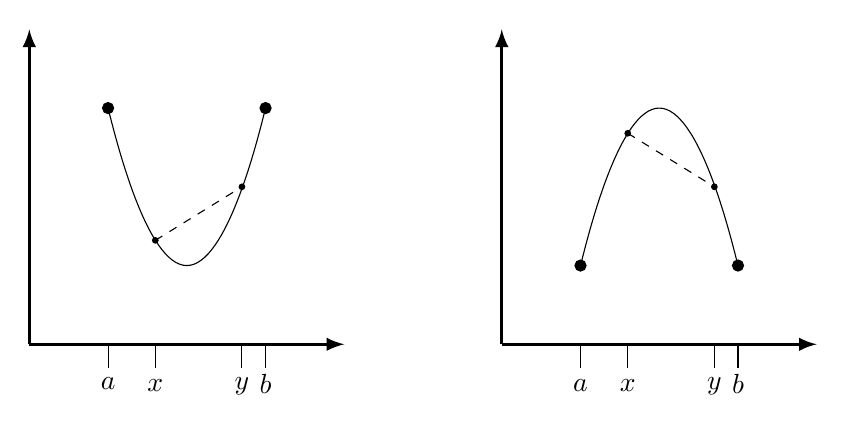
\begin{tikzpicture}[scale=2]
        \draw[-latex, very thick] (-2.5, 0) -- (-2.5, 2);
        \draw[-latex, very thick] (-2.5, 0) -- (-0.5, 0);
        \draw[] (-1.5, 0.5) parabola (-2, 1.5);
        \draw[] (-1.5, 0.5) parabola (-1, 1.5);
        \filldraw[] (-2, 1.5) circle (1pt);
        \filldraw[] (-1, 1.5) circle (1pt);
        \draw[] (-2, 0) -- (-2, -0.15);
        \node[below] at (-2, -0.15) {$a$};
        \draw[] (-1, 0) -- (-1, -0.15);
        \node[below] at (-1, -0.13) {$b$};
        \draw[] (-1.7, 0) -- (-1.7, -0.15);
        \node[below] at (-1.7, -0.16) {$x$};
        \draw[] (-1.15, 0) -- (-1.15, -0.15);
        \node[below] at (-1.15, -0.15) {$y$};
        \filldraw[] (-1.7, 0.66) circle (0.5pt);
        %\node[left] at (-2.5, 0.66) {$f(x)$};
        \filldraw[] (-1.15, 1) circle (0.5pt);
        %\node[left] at (-2.5, 1) {$f(y)$};
        \draw[dashed] (-1.7, 0.66) -- (-1.15, 1);
        \draw[-latex, very thick] (0.5, 0) -- (0.5, 2);
        \draw[-latex, very thick] (0.5, 0) -- (2.5, 0);
        \draw[] (1.5, 1.5) parabola (1, 0.5);
        \draw[] (1.5, 1.5) parabola (2, 0.5);
        \filldraw[] (1, 0.5) circle (1pt);
        \filldraw[] (2, 0.5) circle (1pt);
        \draw[] (1, 0) -- (1, -0.15);
        \node[below] at (1, -0.16) {$a$};
        \draw[] (2, 0) -- (2, -0.15);
        \node[below] at (2, -0.13) {$b$};
        \draw[] (1.3, 0) -- (1.3, -0.15);
        \node[below] at (1.3, -0.16) {$x$};
        \draw[] (1.85, 0) -- (1.85, -0.15);
        \node[below] at (1.85, -0.15) {$y$};
        \filldraw[] (1.3, 1.34) circle (0.5pt);
        \filldraw[] (1.85, 1) circle (0.5pt);
        \draw[dashed] (1.3, 1.34) -- (1.85, 1);
    \end{tikzpicture}
    \caption{Visualization of a convex and non-convex function. For the upwards facing parabola, the function (and hence all points $(\lambda x + (1- \lambda) y, f(\lambda x + (1- \lambda) y))$ for $\lambda \in (0, 1)$) always lies below the line connecting $(x, f(x))$ and $(y, f(y))$ for $a < x < y < b$ and hence it is convex. For the downwards facing parabola, this is no longer true and the function is not convex (it is instead\textit{concave}).}
    \label{fig25}
\end{figure}

\noindent Another equivalent way of defining convexity is to say that $f$ is convex if and only if for all $a < s < t < y < b$:
\begin{align*}
    \frac{f(t) - f(s)}{t - s} \leq \frac{f(u) - f(t)}{u - t}
\end{align*}

\begin{figure}[htbp]
    \centering
    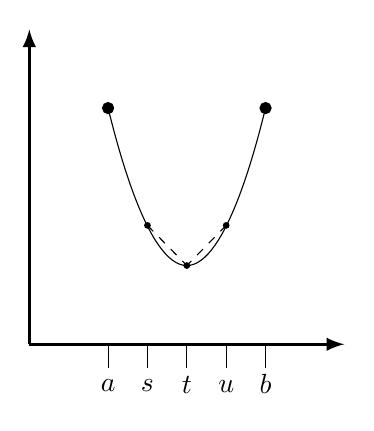
\begin{tikzpicture}[scale=2]
        \draw[-latex, very thick] (0, 0) -- (0, 2);
        \draw[-latex, very thick] (0, 0) -- (2, 0);
        \draw[] (1, 0.5) parabola (0.5, 1.5);
        \draw[] (1, 0.5) parabola (1.5, 1.5);
        \filldraw[] (0.5, 1.5) circle (1pt);
        \filldraw[] (1.5, 1.5) circle (1pt);
        \draw[] (0.5, 0) -- (0.5, -0.15);
        \node[below] at (0.5, -0.16) {$a$};
        \draw[] (1.5, 0) -- (1.5, -0.15);
        \node[below] at (1.5, -0.13) {$b$};
        \draw[] (0.75, 0) -- (0.75, -0.15);
        \node[below] at (0.75, -0.16) {$s$};
        \draw[] (1.25, 0) -- (1.25, -0.15);
        \node[below] at (1.25, -0.17) {$u$};
        \draw[] (1, 0) -- (1, -0.15);
        \node[below] at (1, -0.14) {$t$};
        \filldraw[] (1, 0.5) circle (0.5pt);
        \filldraw[] (0.75, 0.755) circle (0.5pt);
        \filldraw[] (1.25, 0.755) circle (0.5pt);
        \draw[dashed] (0.75, 0.755) -- (1, 0.5);
        \draw[dashed] (1.25, 0.755) -- (1, 0.5);
    \end{tikzpicture}
    
    \caption{Visualization of the alternative definition of convexity. For any $a < s < t < u < v$, the slope of the line segment joining $s$ and $t$ is less than the slope of the line segment joining $t$ and $u$.}
    \label{fig26}
\end{figure}

\begin{ntheorem}{}{}
    \begin{enumerate}[(a)]
        \item Assume that $f: (a, b) \mapsto \RR$ is convex. Then, $f$ is continuous.
        \item Assume that $f \in C^1(a, b)$. Then, if $f$ is convex, $f'$ is increasing.
        \item Assume that $f \in C^2(a, b)$. Then $f$ convex implies $f'' \geq 0$. 
    \end{enumerate}
\end{ntheorem}
\begin{nproof}
    \begin{enumerate}
        \item Let $[c, d] \subset (a, b)$ and $a < c_1 < c < x < y < d < d_1 < b$. By convexity, we have that:
        \begin{align*}
            \frac{f(y) - f(x)}{y - x} \leq \frac{f(d) - f(y)}{d - y} \leq \frac{f(d_1) - f(d)}{d_1 - d}
        \end{align*}
        and also that:
        \begin{align*}
            \frac{f(y) - f(x)}{y - x} \geq \frac{f(x) - f(c)}{x - c} \geq \frac{f(c) - f(c_1)}{c - c_1}
        \end{align*}
        We therefore have that:
        \begin{align*}
            \set{\abs{\frac{f(y) - f(x)}{y - x}}: c < x < y < b} < M
        \end{align*}
        for some $M \in \RR$. Therefore, $\abs{f(y) - f(x)} < M\abs{y - x}$ for all $x, y \in (c, d)$. This holds for all $[c, d] \subset (a, b)$, showing the continuity of $f$.
        \item Let $f$ be convex, and let $a < c < x < y < d < b$. Then, by convexity we have that:
        \begin{align*}
            \frac{f(x) - f(c)}{x - c} \leq \frac{f(y) - f(x)}{y - x} \leq \frac{f(d) - f(y)}{d - y}
        \end{align*}
        Ignoring the central term in the inequality, and taking the limit as $x \rightarrow c$ and $ y \rightarrow b$, we have that:
        \begin{align*}
            f'(c) \leq f'(b)
        \end{align*}
        So we conclude that $f'$ is increasing on $(a, b)$. 
        \item If $f$ is convex, $f'$ is increasing by (b). Then, we have that for any $a < x < y < b$:
        \begin{align*}
            \frac{f(y) - f(x)}{y - x} \geq 0
        \end{align*}
        And hence taking $y \rightarrow x$ we have that $f'(x) \geq 0$. \qed
    \end{enumerate}
\end{nproof}

\begin{ncorollary}{}{}
    If $f \in C^3(I)$ and $f'(x_0) = 0$ and $f''(x_0) \neq 0$, $x_0$ is a local minimum if $f$ is convex in a neighbourhood of $x_0$. 
\end{ncorollary}